\documentclass[12pt, a4paper]{article}
\usepackage{amsmath}
\usepackage{amsfonts}
\usepackage{amsthm}
\usepackage{mathtools}
\newtheorem{theorem}{Theorem}[section]
\newtheorem{definition}{Definition}[section]
\numberwithin{equation}{section}
\usepackage{pgfplots}
\pgfplotsset{width=10cm,compat=1.9}
\graphicspath{ {img/} }
\DeclareGraphicsExtensions{.png}
\DeclareGraphicsExtensions{.jpg}

\title{Single value decomposition and pseudo-inverses}
\author{Kristian Wichmann}

\begin{document}
\maketitle

\section{Gramian matrices}
Given a set of vectors $a_1, a_2,\ldots, a_n\in\mathbb{R}^m$, the Gramian matrix is the traditionally matrix of inner products $\langle a_i,a_j\rangle$. If these vectors are collected into a $m\times  n$ matrix $A$, this matrix can be expressed as $A^t A$. Here, we will use the term for any matrix in this form. By starting out with the transpose instead, this means that $AA^t$ is also a Gramian, with dual results.

\begin{theorem}
If $A\in\mathbb{R}^{m\times n}$, then $A^t A$ is symmetric and positive semi-definite. Iff $A$ has rank $m$, $A^t A$ is positive definite.
\end{theorem}
\begin{proof}
$(A^t A)^t=A^t(A^t)^t=A^t A$ shows symmetry. positive semi-definiteness, let $x\in\mathbb{R}^n$. Then:
\begin{equation}
x^t A^t Ax=\langle Ax,Ax\rangle=||Ax||^2
\end{equation}
As a norm, this is greater than or equal to zero. Hence $A^t A$ is positive semi-definite. If $A$ has rank $m$ the map $x\mapsto Ax$ has a trivial kernel by the rank-kernel theorem. Which means only the zero vector is mapped to zero, and hence $A^t A$ is positive definite. If the rank is less than $m$, the kernel is non-trivial and positive definiteness cannot be true.
\end{proof}

\section{Single value decomposition}
Let $A\in\mathbb{R}^{m\times n}$. Since $A^t A$ is symmetric, it is diagonalizable. So there is an orthogonal $n\times n$ matrix $O$ such that $A^t A=ODO^t$, where $D$ is a diagonal matrix of eigenvalues. 

\begin{figure}
\centering
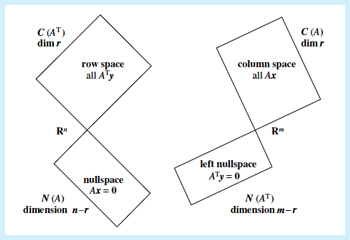
\includegraphics[width=\textwidth]{row_column_null}
\caption{Visualization of dimensionality for the rank-nullity theorem}
\label{fig:rank-nullity}
\end{figure}

\section{Generalized inverses}
For an invertible matrix $A$, it's obviously true that:
\begin{equation}
AA^{-1} A=A
\end{equation}
If $A$ is not invertible, we may still define a \textit{generalized inverse} $A^g$ as a matrix that satisfies the same equation:
\begin{equation}
\label{genralized_inverse}
AA^g A=A
\end{equation}


\subsection{Left and right inverses}
If $A\in\mathbb{R}^{m\times n}$ has rank $n$, then the null space is trivial, and hence the corresponding linear transformation is injective. This means that the equation $Ax=b$ may or may not have a solution, but if it exists, it's unique. The matrix $A^tA$ has rank $n$ as well, and hence is invertible. This can be used to construct a left inverse:
\begin{equation}
A^{-1}_L=(A^t A)^{-1}A^t,\qquad A^{-1}_L A=(A^t A)^{-1}A^t A=I_n
\end{equation}

Similarly, if $A\in\mathbb{R}^{m\times n}$ has rank $m$, then the image space is all of $\mathbb{R}^m$, and hence the corresponding linear transformation is surjective. This means that the equation $Ax=b$ always has a solution, and it may have infinitely many. The matrix $AA^t$ has rank $m$ as well, and hence is invertible. Analogously, we can use this to contruct a right inverse:
\begin{equation}
A^{-1}_R=A^t(AA^t)^{-1},\qquad AA^{-1}_R=AA^t(AA^t)^{-1}=I_m
\end{equation}

Both of of these inverses (when they exist) satisfies equation \ref{genralized_inverse}.

\end{document}